\chapter{Metodología y materiales}
\label{chapter:metodologia}

\chapquote{Caer está permitido, levantarse es obligatorio.}{Proverbio ruso}

En este capítulo, se introducen algunas de las principales metodologías de desarrollo \textit{software} que actualmente más se utilizan.

\section{Metodologías de desarrollo del \textit{software} de Sistemas}

\todo[inline]{añadir tableros  etc}

%Se implementaron los siguientes elementos
%            
%\begin{itemize}
%    \item Tablero Kanban. Aquí son almacenadas las tareas del proyecto, con atributos sobre su estado, su categoría y sus fechas de desarrollo.
%        \begin{figure}[h!]
%            \centering
%            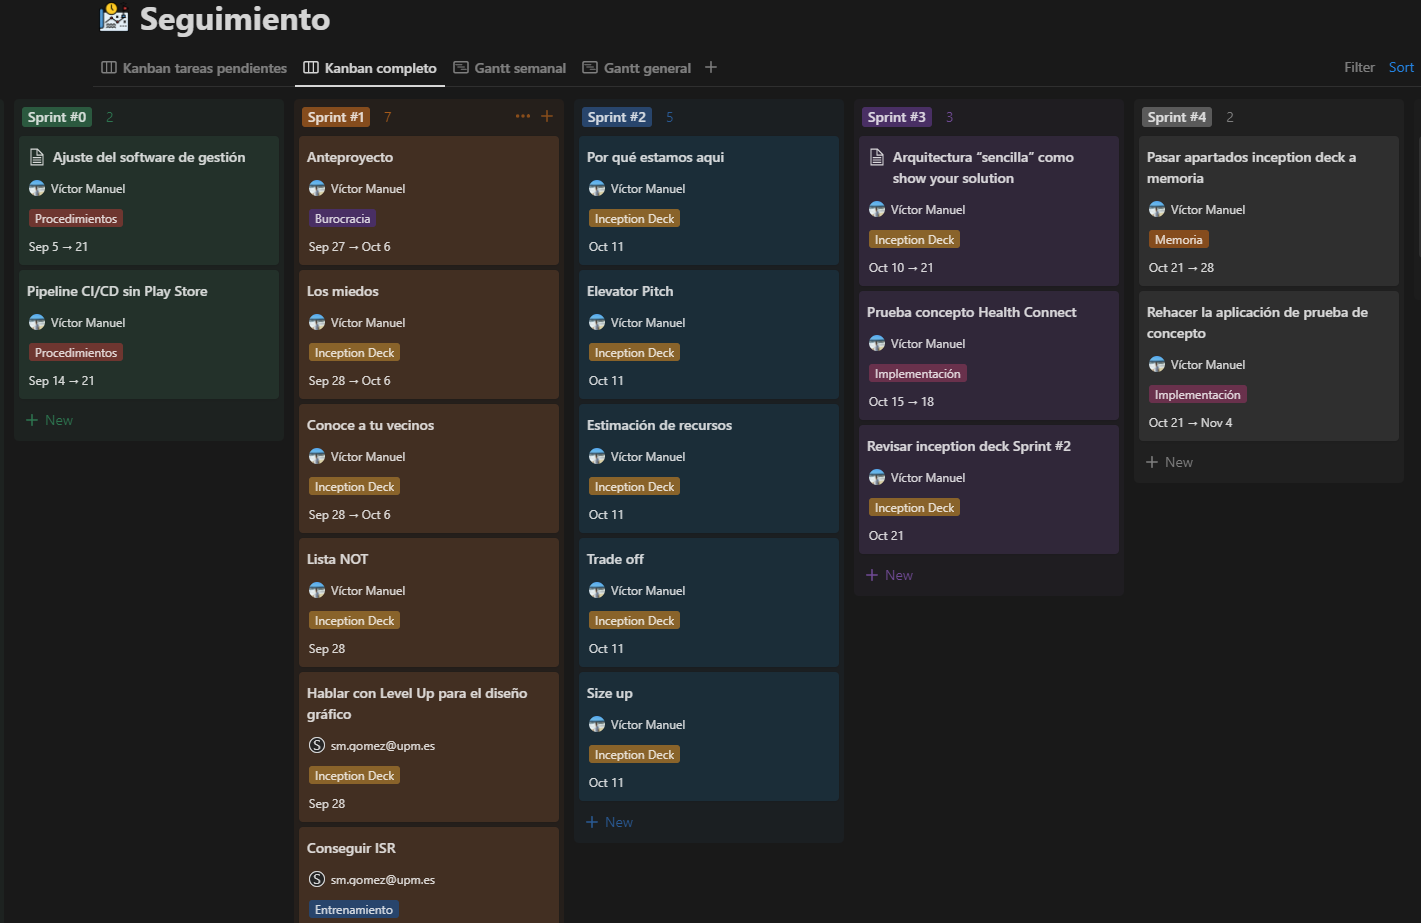
\includegraphics[width=0.75\textwidth]{figures/Kanban completo.PNG}
%            \caption{Extracto del tablero Kanban del proyecto}
%            \label{fig:notion:kanban}
%        \end{figure}
%    \item Diagrama Gantt. En esencia es una vista a la misma base de datos que la del tablero Kanban.
%        \begin{figure}[h!]
%            \centering
%            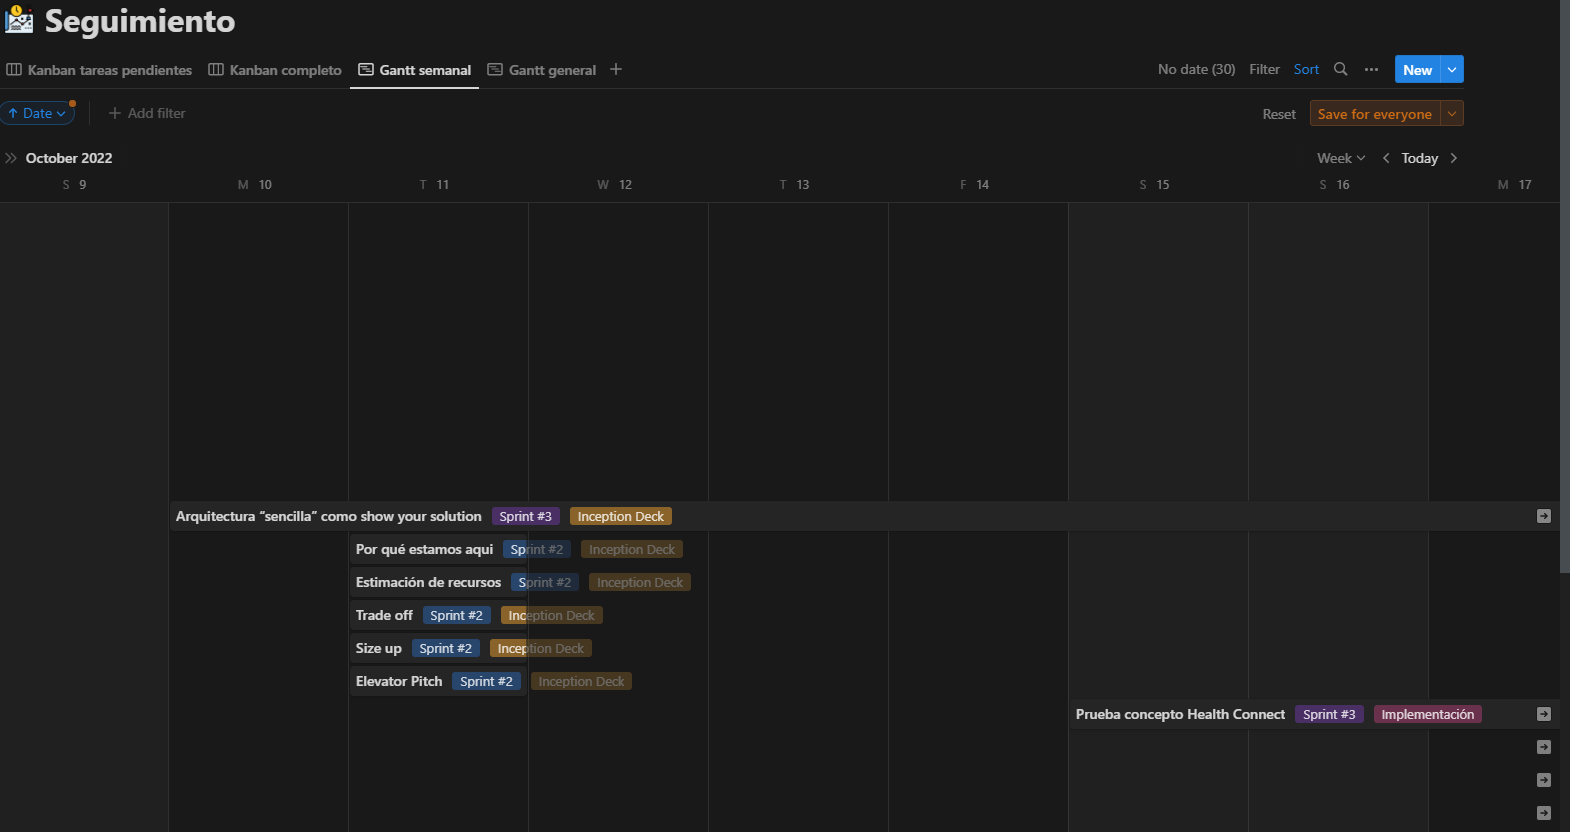
\includegraphics[width=0.75\textwidth]{figures/gantt semanal.PNG}
%            \caption{Extracto del diagrama Gantt del proyecto}
%            \label{fig:notion:gantt}
%        \end{figure}
%    \item Base de datos de referencias con todos los link de interés para la implementación del proyecto. Algunos de ellos aparecen en la bibliografía de esta memoria por su relevancia para exponer ciertas cuestiones.
%        \begin{figure}[h!]
%            \centering
%            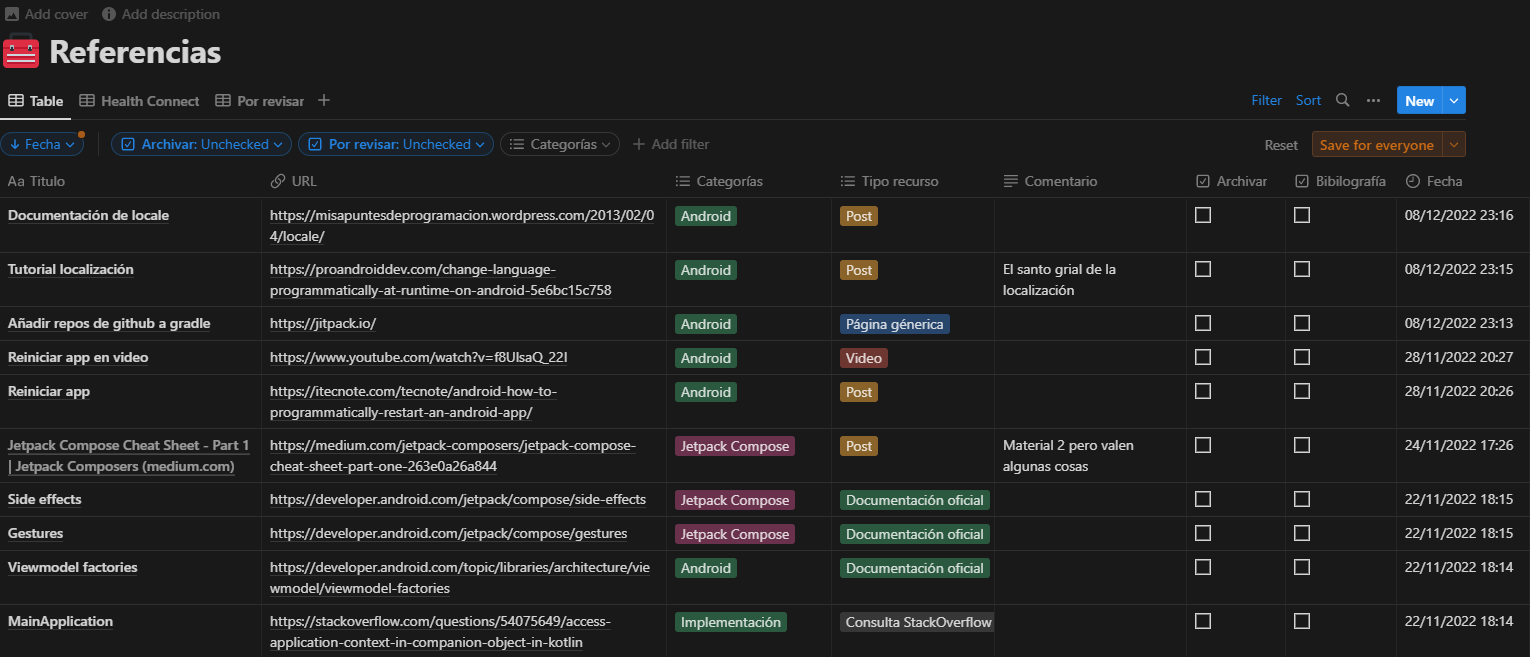
\includegraphics[width=0.75\textwidth]{figures/referencias.PNG}
%            \caption{Extracto de la base de datos de referencias}
%            \label{fig:notion:referencias}
%        \end{figure}
%    \item Base de datos con apuntes de consulta. Aquí se alojan descripciones de conceptos de utilidad para el proyecto. Está enlazada con la base de datos de referencia para acceder rápidamente a los enlaces para ampliar esa información.
%        \begin{figure}[h!]
%            \centering
%            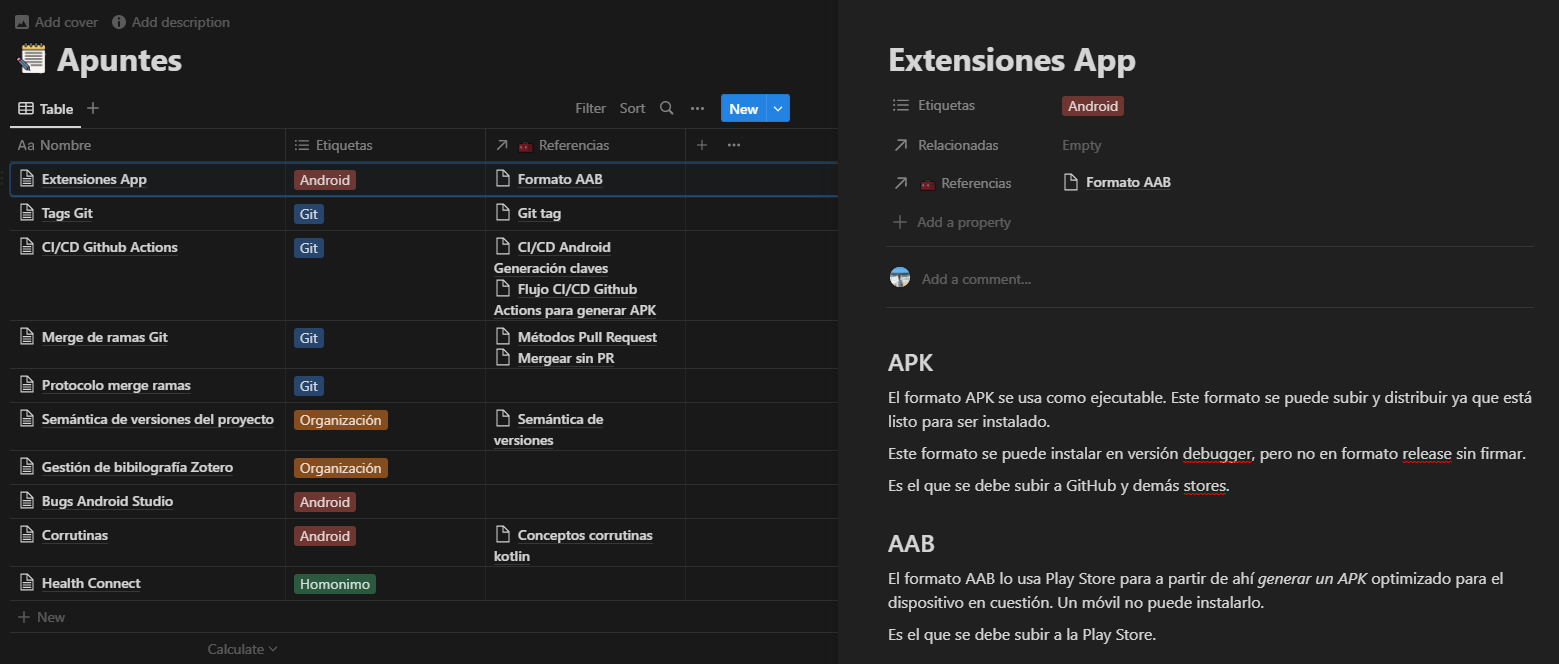
\includegraphics[width=0.75\textwidth]{figures/apuntes.PNG}
%            \caption{Extracto de la base de datos de apuntes del proyecto}
%            \label{fig:notion:apuntes}
%        \end{figure}
%\end{itemize}

\todo[inline]{hablar de los repositorios git y github}

\subsection*{Metodología del desarrollo seleccionada}

PROCEDIMIENTO DE DESARROLLO
Desde un punto de vista ingenieril, la evolución de este Proyecto a través de sus diferentes fases será llevada a cabo siguiendo la metodología de desarrollo en cascada.
Esta metodología, según Ian Somerville, autor del libro Software Engineering (Sommerville, 2011), separa las actividades fundamentales involucradas en cualquier proceso del desarrollo de un software, siendo estas la especificación, desarrollo, validación y evolución, en una secuencia de fases: definición de requerimientos, diseño del sistema software, implementación y prueba de unidad, integración y pruebas del sistema y, por último, operación y mantenimiento. El desarrollo se lleva a cabo completando cada una de estas fases de forma secuencial, pudiendo regresar a cualquiera de las fases anteriores solo tras haber completado previamente la secuencia completa (a cada ciclo a través de estas fases se le conoce como iteración), véase como referencia la Figura 57.
Para el detalle de los conceptos y el procedimiento propuesto por este modelo, se remite al lector a la lectura del primer apartado del capítulo 2, “Software Process Models”, del libro citado anteriormente.
 
Figura 57. Fases del modelo en cascada (Sommerville, 2011).
Trasladando los conceptos propuestos por esta metodología al contexto del desarrollo de un sistema de software basado en DL, la fase de implementación correspondería con el entrenamiento del modelo y la fase de prueba con la validación de este, el resto de las fases permanecerían igual.
El uso de otras metodologías tradicionales, como el desarrollo incremental y el desarrollo orientado a la reutilización (puede encontrase también la explicación sobre ambas en el libro citado en el párrafo anterior en el capítulo 2, “Modelos de Proceso de Software”), han sido descartadas. Por un lado, el desarrollo incremental no es necesario para este Proyecto, pues el sistema final que se pretende lograr con este Proyecto no surge como el resultado de integrar funcionalidades de forma progresiva, sino que este es concebido como un conjunto de partes que deben ser acopladas al mismo tiempo, el análisis multimodal de diferentes fuentes de información y la combinación de estos resultados individuales mediante la fusión multimodal para la construcción de un sistema basado en diversos modelos entrenado y probado como un todo no puede segregarse como partes individuales pues carecería de sentido para tal propósito.
Por otro lado, el desarrollo orientado a la reutilización tampoco se adapta al contexto de este Proyecto, pues al tratarse de un ámbito de aplicación tan específico como lo es el diagnóstico de la depresión a través del DL, los componentes reutilizables no existen como tal, es cierto que existe código ya implementado como parte de la realización de estudios similares, pero estas implementaciones, a pesar de ser reproducibles, están lejos de haber sido diseñadas con la finalidad de ser reusadas para otros usos, pues la reutilización no suele ser uno de los objetivos en trabajos de investigación ligados a contextos tan concretos como el de este Proyecto. A pesar de ello, sí serán usadas algunas librerías y herramientas ya desarrolladas para implementar el software de este Proyecto, si bien, el rol de ambas será totalmente secundario pues servirán únicamente al propósito de implementación de este software y no a la materialización de la funcionalidad requerida, y, como tal, no será conveniente orientar el desarrollo entorno al uso de estas.
Otra alternativa, serían las metodologías ágiles, no obstante, estas parecen proveer un ecosistema de desarrollo no tan maduro y poco apto para tareas de DL. En un estudio publicado por Kushal Singla, Joy Bose y Chetan Naik en el año 2018 (Singla et al., 2018), se analiza la aplicación del procedimiento de desarrollo Scrum, una de las metodologías ágiles más populares, en diversos proyectos que involucran procesos de ML. La conclusión a la que llegaron con su investigación es que Scrum, y las metodologías ágiles en general, parecen no adaptarse completamente a las necesidades particulares que surgen del uso de la IA para la resolución de problemas. Uno de los mayores defectos es la dificultad de predecir el tiempo requerido para ejecutar cada una de las tareas típicas en el marco del ML. En el mismo estudio, los autores sugieren ciertas sugerencias para atajar estos defectos, aunque, desafortunadamente, un estudio de la efectividad de dichas recomendaciones todavía no ha sido concretado. En definitiva, una metodología ágil contrastada y diseñada específicamente para trabajos con IA es algo que aún queda pendiente por resolver.



%Texto :
%1. Rn la Fase de análisis se va a hacer x,yz.
%2. En la Fase 